\newpage
\section{Constructive heuristics}

% Introduzione
\subsection{Introduzione}
Nel (caso peggiore) di variabili binarie il livello computazionale sarà dato da $O(2^n)$ quindi il tempo di calcolo cresce esponenzialmente con il numero di variabili. 

In molte applicazioni si fa affidamento ad \hl{algoritmi detti inesatti} che \hl{CERCANO di generare delle soluzioni ammissibili}. Questi rientrano negli \hl{algoritmi euristici} dove è importante che la \hl{conoscenza del progettista venga trasmessa all'algoritmo}. Questi algoritmi possono essere:

\begin{itemize}
    \item \textbf{costruttivi}: dove \hl{cercano di generare una prima soluzione ammisibile}
    \item \textbf{migliorativi}: dove \hl{prova a migliorare la prima soluzione}
\end{itemize}

Trovare una soluzione ammissibile potrebbe essere difficile dato che potrebbe essere più complicato del trovarne una ottima.


% Travellig Salesman Problem (TSP)
\subsection{Travellig Salesman Problem (TSP)}

Data una matrice $C$ di transizione dove, per andare dal punto $1$ al $2$ \hl{pago $c_{12}$} e così via per tutte le possiabili iterazioni \hl{per un numero $n$ di punti da "visitare"}. Lo scopo sarebbe trovare un circuito che tocchi tutti i punti una sola volta con \hl{costo minimo}.

Avremo che il \hl{tempo di ciclo determina la produttivita' della macchina} tipo un robot che fa n fori e conclusi gli n fori finisce oil cilo.

Un vincolo ulteriore potrebbero essere le \hl{finestre temporali} che potrebbero esserci come nei casi di consegna dei pacchi amazon, il che \hl{rende computazionalmente piu' difficile o anche inammissibile il problema}. Notare come cambiando anche solo un dato potremmo avere una soluzione ammsisibile o una crescita esposnenziale dell'infattibilità dala quele deriva l'instabilità.


% Algoritmo greedy
\subsection{Algoritmo Greedy}

Algoritmo che \hl{cerca di massimizzare nel breve periodo} (usato per essere adattato a qualsiasi problema). È un'\hl{euristica di tipo costruttivo}, infatti ha una \hl{procedura sequenziale} che costruisce la soluzione passo passo \hl{massimizzando solo l'utilizzo immediato} andando però in contro a:

\begin{itemize}
    \item una soluzione inammissibile
    \item non garantire una soluzione ottima
\end{itemize}

il suo \hl{pseudocodice} è un adattamenteo sull'algoritmo del Travellig Salesman Problem (TSP):

\begin{itemize}
    \item[] last = 1 (last = ultimo punto toccato)
    \item[] $S = \{2,3,...,n\}$
    \item[] while ($S \neq$ insieme vuoto)
    \begin{itemize}
        \item[] estrarre da $S$ un punto
        \begin{itemize}
            \item[] $i = \text{argmin}_{i \in S} c_{\text{last}, i}$
            \item[] $\text{succ}_{last} = i$
            \item[] last $= i$
        \end{itemize}
    \end{itemize}
    \item[] $\text{succ}_{last} = 1$ 
\end{itemize}

Vediamo un esempio con dati: $n = 4$ e
$$C=
\left[ {\begin{array}{cccc}
    0 & 10 & 5 & 8 \\
    10 & 0 & 2 & 1 \\
    5 & 2 & 0 & 4 \\
    8 & 1 & 4 & 0 \\
\end{array} } \right]
$$

dove applicando l'algoritmo abbiamo:

\begin{itemize}
    \item last = 1; $\rho = <2,3,4>$
    \item last = 3 ; $\rho=<2,4>$; $\text{succ}_1 = 3$
    \item last = 2; $\rho=<4>$; $\text{succ}_3 = 2$
    \item last = 4; $\rho =<>$; $\text{succ}_2 =4$
    \item $\text{succ}_4 = 1$
\end{itemize}


% Miller-Tucker-Zemlin
\subsection{Miller-Tucker-Zemlin}

Questo modello definisce delle \hl{variabili binare $x_{ij}$} per ogni coppia di punti $i$ e $j$:

$$ x_{ij} =
\begin{cases} 
    1, \text{ se } i,\ j \text{ sono/saranno visitati} \\ 
    0, \text{altrimenti}
\end{cases}
$$

avremo allora che:
$$\min \sum_{i,j} c_{i,j} x_{i,j}$$
s.t
\begin{itemize}
    \item $\sum{j} x_{ij} = 1\ \ \ \forall i$
    \item $\sum{j} x_{ji} = 1\ \ \ \forall i\ ->$ dice che ogni punto ha un suo successore
    \item $0 \leq x_{ij} \leq 1\ \ \ \forall x_{ij} \text{ integer} ->$ dice ogni punto ha un predecessore
\end{itemize}

Questi \hl{vincoli non bastano} per poter risolvere il modello, infatti non possiamo escludere di avere una \hl{soluzione disconnessa (sub-tour)}


\begin{figure}[H]
\centering
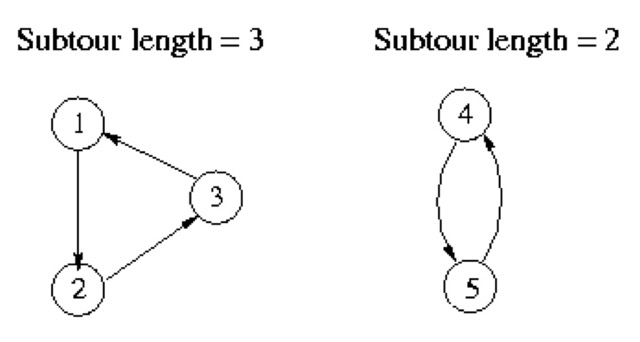
\includegraphics[scale=0.3]{sep.jpeg}
\caption{Soluzione disconnessa} 
\label{sep}
\end{figure}


Si introducono allora dei \hl{vincoli di connessione} della soluzione tramite una \hl{variabile per l'ordine di vista: $u_i$} (una per ogni punto).

Poniamo allora un punto iniziale con $u_i = 1$:

\begin{itemize}
    \item[] $u_1 = 1 -> x_{1,3} = 1$
    \item[] $u_3 = 2 -> x_{3,4} = 1$
    \item[] $u_4 = 3 -> x_{4,2} = 1$
    \item[] $u_2 = 4 -> x_{2,1} = 1$
\end{itemize}

altri \hl{vincoli da imporre su $u_i$}:

\begin{itemize}
    \item $2 \leq u_i \leq 1\ \ \ \forall i \neq 1$
    \item $u_i - u_j + 1 <= n(1-x_{ij})\ \ \ \forall i,j \neq 1$
\end{itemize}

Avremo quidni \hl{2 casi}:

\begin{itemize}
    \item $x_{ij} = 0\ \Rightarrow\ u_i - u_j +1 \leq n$: ovvio dato che tutte le variabili \textbf{$u$ sono comprese in $n$}
    \item $x_{ij} = 1\ \Rightarrow\ u_i - u_j + 1 \leq 0$: dato che $u_j \geq u_i + 1$ allora \textbf{$i$ predecessore di $j$}
\end{itemize}


% Algoritmo relax-and-fix
\subsection{Algoritmo relax-and-fix}

Si usa per \hl{problemi multiperiodali} dato che voglio poter avere un approccio con \hl{suddivisione in piu' periodi temporali}:

$$\min z = c^Tx$$
s.a.
\begin{itemize}
    \item $Ax=b$
    \item $x \geq 0$ (integer)
\end{itemize}

\hl{Partiziono le variabli in $n$ gruppi} in modo da avere variabili impiegate per un solo intervallo di tempo. Allora il problema diventa:

abbiamo alloradelle applicazioni ndove le varaibili naturalemte si dividono in gruppi datoun osviluppo temporale, il orblema allora diventa:

$$\min z = \sum_{i=1}^n c_i^Tx_i$$
s.a.
\begin{itemize}
    \item $\sum_{i=1}^na_ix_i=b$
    \item $x_i \geq 0$ (integer)
\end{itemize}

la difficoltà del problema si trova nelle molte varibili intere. Posso allora \hl{definire un problema con variaibli $x_1$ del primo gurppo intere}, per le restanti faccio un rilassamento. Potremo avere che:


\begin{itemize}
    \item ausiliario: inammissibile $\to$ iniziale: inammissibile
    \item ausiliario: sol. ottima $\to$ fisso $x_1$ alla soluzione: $x_1 = \overline{x}_1$
\end{itemize}

Quindi per \hl{risolvere il problema} dobbiamo:

\begin{enumerate}
    \item $\underline{x}_1$ diventa \textbf{intera}
    \begin{itemize}
        \item \textbf{rilasso} le altre variabili
        \item \textbf{risolvo} il problema e \textbf{fissiamo} $x_1 = \overline{x}_1$ che viene "rimossa" dal modello
    \end{itemize}

    \item ecc, ecc...
\end{enumerate}

Così facendo \hl{tengo conto delle variabili "future"} senza richiede un grande sforzo computazione, dato che lavora sul singolo gruppo.

\hl{Generallizzando}:
$$\min x = \sum_{i=1}^{k-1} c_i \overline{x}_i + c_k x_k + \sum_{i=k+1}^n c_i x+i$$
s.t

\begin{itemize}
    \item $\sum_{i=1}^{k-1} a_i \overline{x}_i + a+k x+k + \sum_{i=k+1}^n a_i x_i = b$
    \item $x_k \geq 0$ (integer)
    \item $x_i \geq 0$
\end{itemize}

Lo \hl{pseudocodice} sarà:

\begin{itemize}
    \item[] found = true
    \item[] for (k = 1 $\to$ n):
    \begin{itemize}
        \item[] solve $P_k(\overline{x}_1,...,\overline{x}_{k-1})$
        \item[] if è inammissibile:
        \begin{itemize}
            \item[] found = false
            \item[] break;
        \end{itemize}
        \item[] else: $(x'_{k+1},...,x'_n)$ è soluzione
        fissare $\overline{x}_k = x'_{k}$
    \end{itemize}
\end{itemize}


% Algoritmo rolling horizon
\subsection{Algoritmo rolling horizon}

Durante il primo periodo considero di:

\begin{enumerate}
    \item creare un \hl{sottoproblema con alcune variabili} da $x_1$ a $x_k$
    \item \hl{trascurare le variabili dei periodi successivi}
    \item fisso $x_1$
    \item mi \hl{muovo di uno step}
    \item considero un \hl{sottoproblema con $x_1$}
    \item \hl{fisso $x_2$} e considero le variabili fino a $x_k+1$.
    \item ecc, ecc...
\end{enumerate}

Andiamo quindi a \hl{risolvere un problema a $k$ variabili} ma \hl{senza tenere in conto le variabili troppo successive}, quindi sarà meno accurato.


% Multiple criteria decision making
\subsection{Multiple criteria decision making}

Spesso abbiamo \hl{piu' obbiettivi} e \hl{non riusciamo a scegliere in anticipo quale ha priorita'} allora spesso vanno in \hl{conflitto}, allora cerchiamo di trovare le migliori soluzioni che devono \hl{rispettare alcuni vincoli}:

$$p \text{ criteria } =
\begin{cases} 
    z_1 = f_1(x) \text{ da }\min \text{ o }\max \\ 
    z_2 = f_2(x) \text{ da }\min \text{ o }\max \\ 
    ... \\
    z_p = f_p(x) \text{ da }\min \text{ o }\max
\end{cases}
$$
s.t

\begin{itemize}
    \item $g(x) \geq 0$
    \item $x \geq 0$
\end{itemize}


Preso un problema di schediling:
abiamo n attivita e come paramentri:
$S_i$ starting time dell'attivita i
$d_i$ durata dell'attivita i
$pij = 1$ se l'attivta j è prerequinistito dell'attivita i, $=0$ altrimenti

obiettivo: minimizare il tempo di completamento = T


avremo allora che:
$min T$
s.t.
$T >= S_i + d_i ....$



formulare un attivta in modo fattiibile:
$D_i$ max durata dell'attivita i
$b_i$ min durata dell'attivita i
$d_i$ durata dell'attivita i
$X_i$ costo per accellerare il comletamento dell'attivita i

allora:
$d_i = D_i-a_iX_i$ con $a_i$ coefficente di ...
...

allora bbiamo da minimizzare 2 obiettivi:
$min \sum .....$
$min T$
s.t.
.....


considerato un oroibkem acon piu obiettvi allor apossimo consederaene uno con obiettivo singolo. quindi le soluzioni ottimali dei singoli porblemi per rappresentarle scrivo nello spazio ammissibile, lo spazio dei criteri rappresentando i singoli obiettivi. a volte puo succedere che presi i du epunto la loro unione non fa parte della zona ammissibile (utopia)

img

ma noi allora adiamo a prendere il punto migiore nella zona ammissibile come in questo caso C dato che è migliore di A per certe cose e per altre rispetto a B

potrmo prender per o un punto D che saràpegio re rispetto ad entrambi gil obiettivi dato che son osoluiozni dominate dareo che f1(D) >= f1(C), e f2(D) >= f2(C)

a noi interesse di trovare le soluzioni non inferioir e quindi efficienti e dobbiamo traovare tra tutte la migliore. per capire qual è quella migliore dipende dal 


si usa allor aun trade off ratio dove prendiamo le soluzioni A e B e calcolipmo il rapporto di trade off facendo:
....

che rappresenta il miglioramento dell'obiettivo iesimo in base al miglioramentodi un altro obiettivo ?!

noi allora ci interessiamok delle soluzioni sulle frontiere dato ceh quel einterne sono dominate da altre piu vicine alla frontiera

se abbiamo una zona convessa avremo che si collegherà in modo immaginario i punti togliendo la convessità e quindi prendiamo i punti sulla forntiera tranne sulla parte immaginaria


per trovare le soluzioni effcienti abbiamo 2 metodi:
- metodo dei vincoli-
- metodo dei pesi


1. prendiamo iun singolo obiettivp e per gli altri imponiamo una soglia dove per ogni obbiettco diverso da quello scelto la funzione obiettivo si a al amssismo:
fk(x) <= uk (dato che minimizziamo)
.....

img


es: nel caso di multischeduling:
vogli ominimizzare il costo come obiettivo, impongo poi un valore soglia al tempo di compeltamento:
$T <= T^*$

con $T^*$ tra Tmin e Tmax in base al fatto che se vogliamo minimizzare o massimizzare



altro metodo: dei pesi:
abbimao una sola f.o. come somma pesate degli altri obiettv:
$\sum wi fi$

com wi obiettivo: 'sum wi = 1

a seconda del valore che diamo ai pesi andiamo a sposatre la retta trangente alla zona ammissibile

img

questo non funziona se è convesso dato che non possiamo traovare tutte le possibili soluzioni dato che la forntiera non è connessa. 

es: con multiobeittvio:
min.....





per scegliere tra le diverse soluzione e traovare quella migliore, dipende dalle preferenze che posson essere espresse tramite una funzione che a seconda de valore dei diversiobiettivi assume un valore di verso allora traovando la suozlione che massimizza il valore della funzioen traviamo al soluzione migliroe per il decisore, il problemaè che in gere non c'è una sluzione matematica per questa cosa ma  posiiamo:
max U ....
s.t.
g(x) >= 0
x >= 0

metodo a priori
se disponiamo di questa funzione in forma chiusa possiamo risolvere i lproblema monoobeittivo masismizzando la funzione (detto metodo a propri)

in genre ono si trova questa solzione

es: settiamo una soglia erapprensetiamko la distaza di f.o. e la soglia adeguata. al variare di r avremo  3 tipi di metriche:
- r=1 ....
- r=2 metrica euclidea ....
- r=+infty .....

sara difficile di re per ogni obeittvi oquale puo esser una solgia adeguata dato che spesso traovare singoli ottimi è complicato.




altro apporccio: a posteriori
andiamoa a genreare tutte le soluzioni effcienti e dire quale tra le soluzione è la migliore. è difficiel applicare al metodo perchè potrebbe cresce in maniera espoenziale con la dimensione del problema



allora usiamo un approccio interattivo:
approccio di mezzo
presi 2 obiettvi troviamo il punto ottimko per entrambi e poi troviamo la priam soluzioneefficiente che si atra A e B e poi si scegli a su quale parte della forntiera vogliamo posizionia=arci. es parte AB e trbiamo una oluizone efficente tra le 2 ecc ecc
 
img

mi fermo quando il segmento che mi rimane è cosi piccolo che i due punti con=incidono

m isposto in base a cosa mi server